\documentclass{article}
\usepackage[T1]{fontenc}
\usepackage[utf8]{inputenc}
\usepackage{hyperref}
\usepackage{graphicx}
\usepackage{caption}
\usepackage{subcaption}
\usepackage{array}
\usepackage{geometry}
\usepackage{amsfonts}

\title{Parallel programming for HPC: exam project\\ Exercise 2: Jacobi method for solving Laplace equation}
\author{\textbf{Student:} Isac Pasianotto}
\date{2024-05}

\setcounter{section}{-1} % Start chapter numbering from 0
\renewcommand{\thesection}{\arabic{section}} % Adjust section numbering in the table of contents

\begin{document}
    \maketitle
    %\tableofcontents

    \section{Requirements}

    The task this assignment aims to take an already existing code that solves the Laplace equation using the Jacobi method, and port it on GPU using \texttt{openACC}.

    \noindent The given \texttt{C} code is write to run on a serial context, hence also the parallelization among different threads is required.

   \section{Implementation}

    In the attempt to exploit as much as possible the resources in which the code is running, the code has been modified, both for the GPU and CPU,
    to run in parallel using \texttt{openMP}, \texttt{openMPI} and \texttt{openACC}.

    \noindent The code now has the following structure:

% Note: the verbatim identation starts from the first character of the line
    \begin{verbatim}
Initialize the local_matrix                                                    [cpu]
Copy the local_matrix to the device                                            [cpu→gpu]
Loop over the number of iterations
    MPI communication to exchange needed cells among the processes              [gpu]
    Compute the new values of the local_matrix                                  [gpu]
Copy the local_matrix back to the host                                          [gpu→cpu]
Write the results to the output file                                            [cpu]
    \end{verbatim}

    The processes in this setting does not allocate the entire matrix, but only a subset of its rows.
    The distribution of rows among the processes is as much as possible uniform, in the case the number of rows is not divisible by the number of processes,
    the remaining rows are distributed among the first processes.

    \noindent In order to compute the values for the next iteration, each process needs to know the values of the cells in the row
    above and below the ones it has.
    This is achieved with the MPI communication.

    In the case the code is executed on nodes equipped with GPUs, the local matrix (and another matrix for the next iteration)
    is copied to the device, and the MPI communication is done from one device to another.
    At the end of each iteration the two matrices pointer are swapped, and the program is ready for the next iteration.

    \noindent Once the loop is completed, the local matrices are copied back to the host, and the results are stored in the output file.
    If for some reason, we need to check the output file, the code can be compiled with removing the \texttt{-DFASTOUTPUT} flag.
    If this is the case, all the processes will perform an MPI\_Gather to the root process, which will write the results to the output file.
    Otherwise, the file will be generated as a binary file, using \texttt{MPI\_IO}, which is extremely faster and more likely to be used in a real scenario.

    \section{Results}

    As requested, I have performed the scaling tests in the following two scenarios:

    \begin{itemize}
        \itemsep0em
        \item \textit{Matrix size:} $1,200 \times 1,200$, \textit{Iterations:} $10$
        \item \textit{Matrix size:} $12,000 \times 12,000$, \textit{Iterations:} $10$
    \end{itemize}

    The code was run on th \href{https://leonardo-supercomputer.cineca.eu/}{Leonardo} cluster in the following way:

    \begin{itemize}
        \itemsep0em
        \item On \href{https://wiki.u-gov.it/confluence/display/SCAIUS/UG3.2.2%3A+LEONARDO+DCGP+UserGuide}{DCGP} nodes, which are used for CPU computing,
             spawning one MPI process per node, and let OpenMP to use all the available cores in the node.
        \item On \href{https://wiki.u-gov.it/confluence/display/SCAIUS/UG3.2.1%3A+LEONARDO+Booster+UserGuide}{Booster} nodes, which are used for GPU computing,
             spawning four MPI processes per node, in this way the program will use all the available GPUs in the node (every task will be pinned to a different GPU).
    \end{itemize}


    The results are represented in the plots in the following pages, but can be summarized as follows:

    \begin{itemize}
        \itemsep0em
        \item If the code is run for a matrix with a size which is too small, it does not scale, and even worse, the overhead introduced by the MPI communication
            makes the code slower than the serial version.
            This is true for both the CPU and GPU version, in the latter case this is even more evident.
        \item For the larger matrix, the code scales well, for both the CPU and GPU version.
        \item Increasing even more the number of node will lead asymptotically in a situation in which the code will
            not scale anymore, and the bottleneck will be the MPI communication.
            This point is reached earlier in the GPU version, due to the fact that the GPU is faster than the CPU and the computation time tends to zero faster.
        \item As expected, running the code on the GPU is faster than on the CPU, but the difference between the two becomes less evident as the number of nodes increases.
    \end{itemize}

    \newpage

    \begin{figure}
        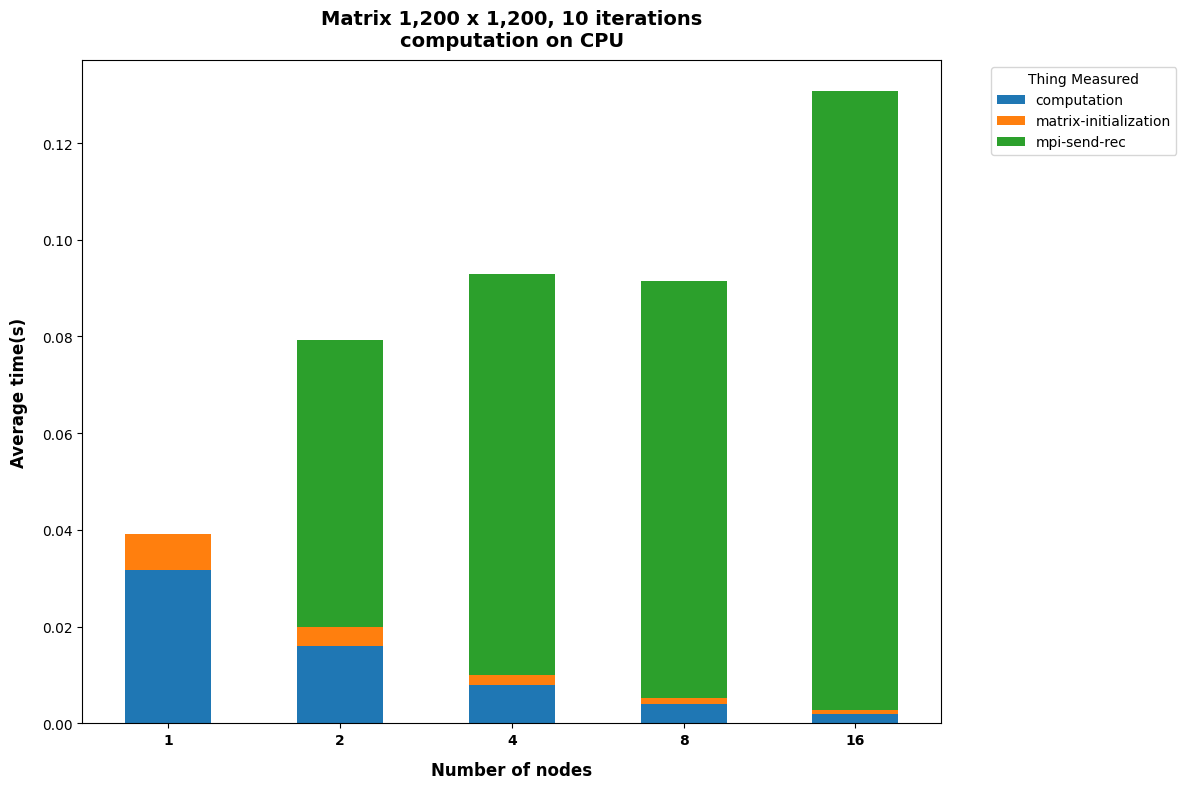
\includegraphics[width=\textwidth]{./plots/plt00}
        \caption{Matrix size: $1,200 \times 1,200$, Iterations: $10$ on CPU.\\ We can see that even if the computation timescale, the overhead introduced by the MPI communication makes the code slower than the serial version.}
        \label{fig:figure0}
    \end{figure}

    \begin{figure}
        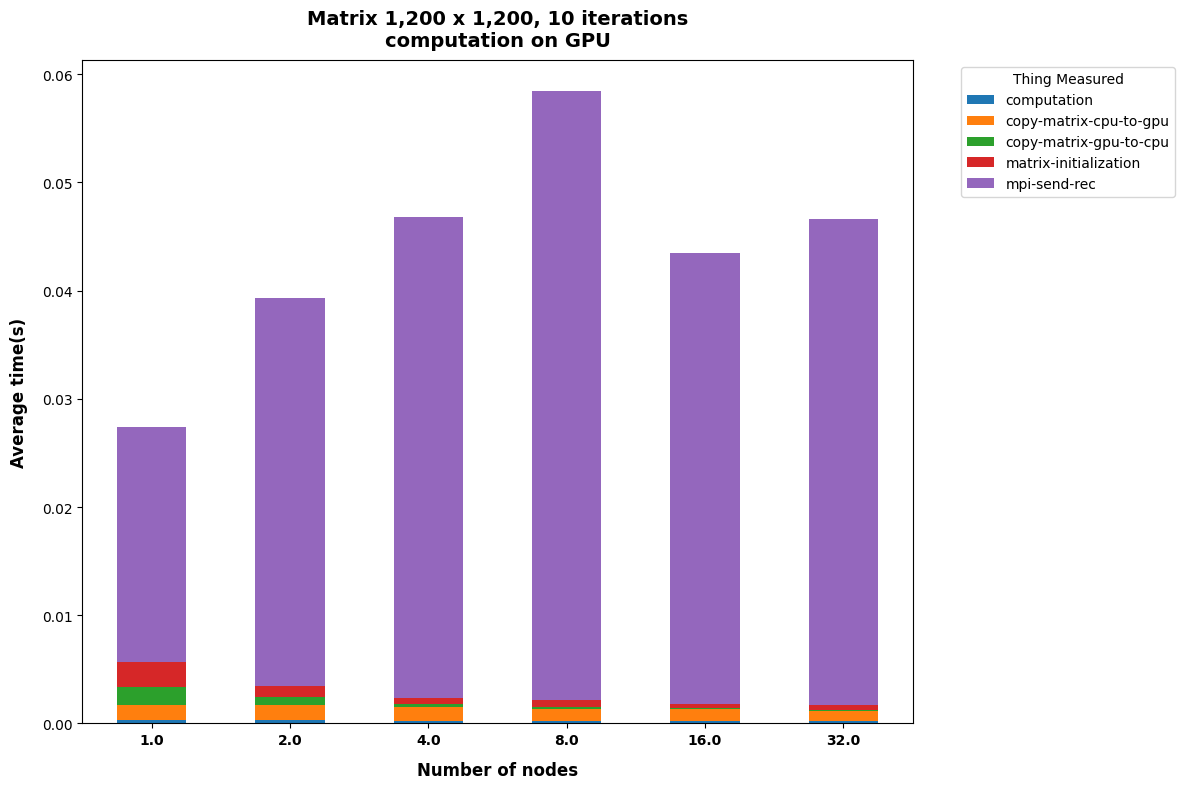
\includegraphics[width=\textwidth]{./plots/plt02}
        \caption{Matrix size: $1,200 \times 1,200$, Iterations: $10$ on GPU.\\ The situation is the same as the CPU version, and it is even more evident.}
        \label{fig:figure1}
    \end{figure}

    \begin{figure}
        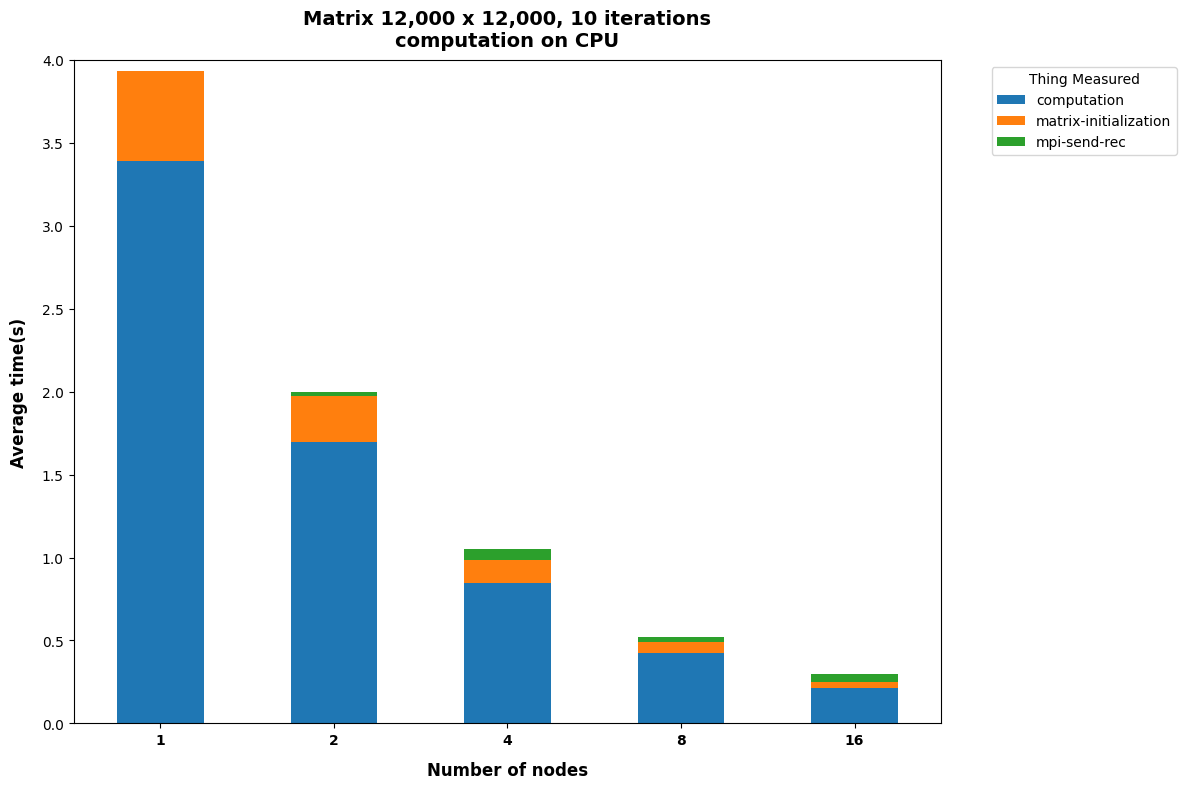
\includegraphics[width=\textwidth]{./plots/plt01}
        \caption{Matrix size: $12,000 \times 12,000$, Iterations: $10$ on CPU.\\ The code scales well, and the computation time tends to zero as the number of nodes increases.}
        \label{fig:figure2}
    \end{figure}

    \begin{figure}
        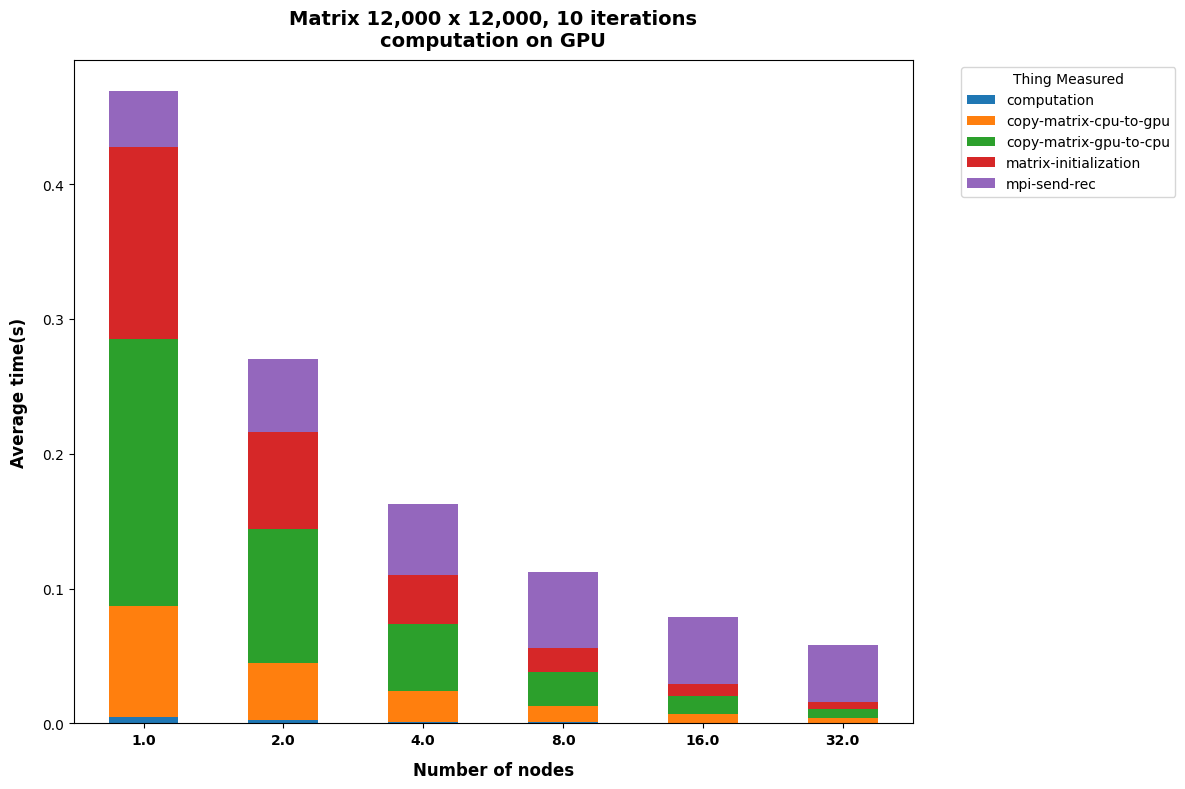
\includegraphics[width=\textwidth]{./plots/plt03}
        \caption{Matrix size: $12,000 \times 12,000$, Iterations: $10$ on GPU.\\ The code scales well, but the computation time tends to zero faster than the CPU version but the overhead introduced by the MPI communication is more evident, probably due to the fact that there are 4 MPI process per node.}
        \label{fig:figure3}
    \end{figure}

    \begin{figure}
        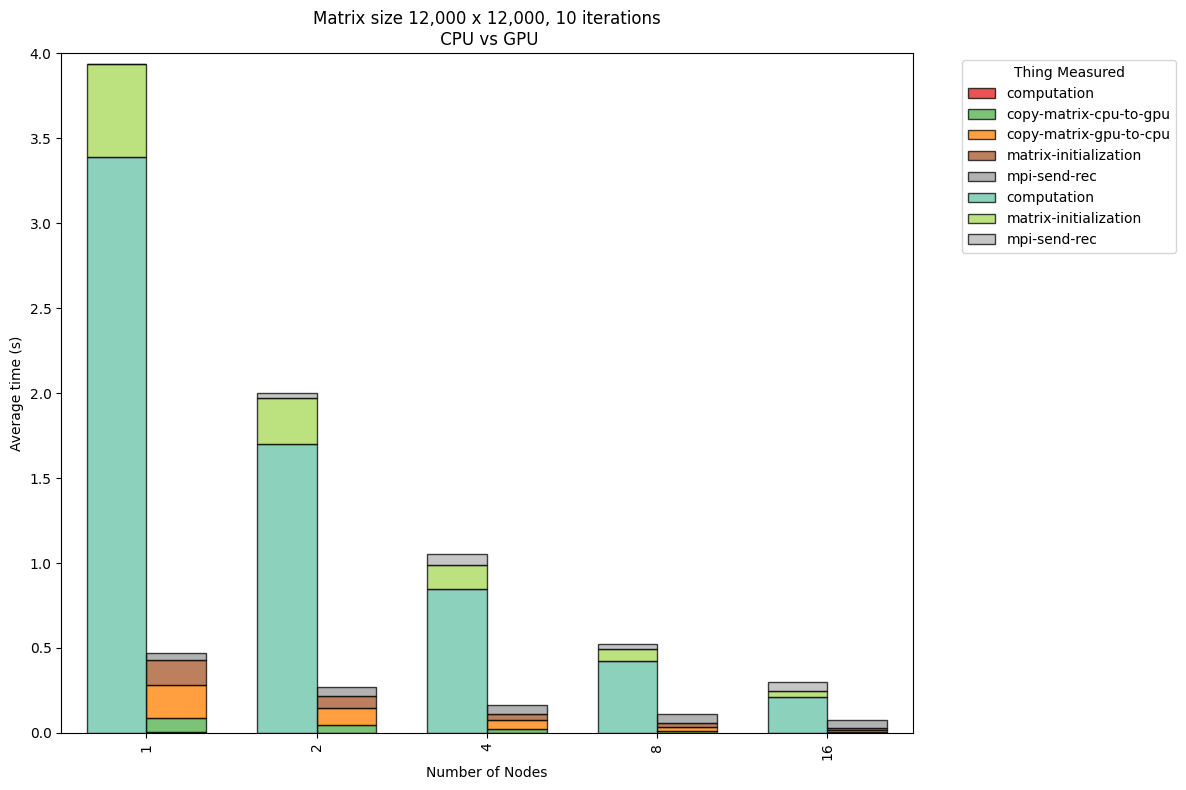
\includegraphics[width=\textwidth]{./plots/plt05}
        \caption{Matrix size: $12,000 \times 12,000$, Iterations: $10$ on CPU and GPU.\\ We can see that the GPU version is faster than the CPU version, but the difference between the two becomes less evident as the number of nodes increases.}
        \label{fig:figure4}
    \end{figure}

    \begin{figure}
        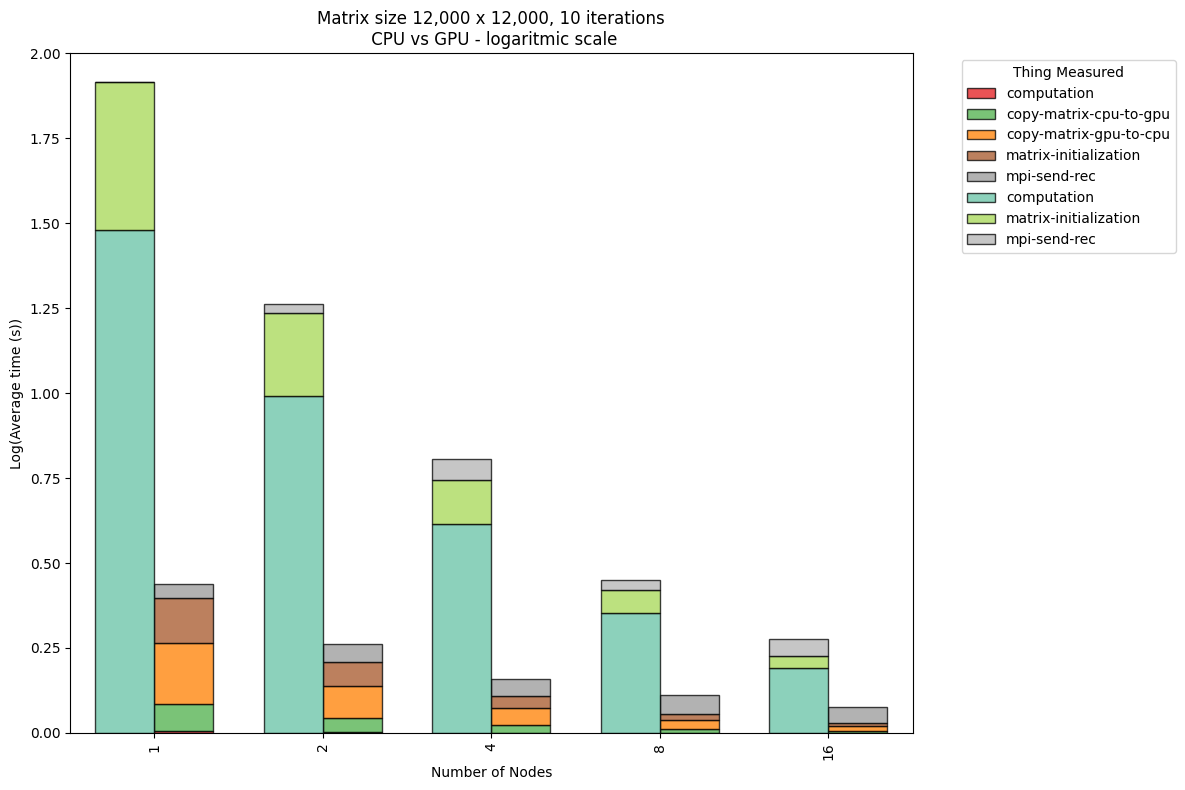
\includegraphics[width=\textwidth]{./plots/plt06}
        \caption{Same as fig.\ref{fig:figure4}, but with a logarithmic scale on the y-axis to better appreciate the different coponents of the stack plot.}
        \label{fig:figure5}
    \end{figure}

\end{document}
